\documentclass[10pt]{article}

\usepackage[margin=1in]{geometry}
\usepackage[utf8]{inputenc}
\usepackage[english]{babel}

\usepackage{algorithm}
\usepackage{algpseudocode}

\usepackage{booktabs}
\usepackage{enumitem}

\usepackage{graphicx}
\usepackage{subcaption}

\usepackage{mathtools}
\usepackage{bm}
\usepackage{siunitx}

\graphicspath{{figs/}}
\sisetup{output-exponent-marker=\ensuremath{\mathrm{e}}}

% Information for header.
\title{Estimating Planetary Habitability via Particle Swarm Optimization of CES Production Functions.}
\author{Abhijit J.\ Theophilus}
\date{\today}

% Useful for initial drafts.
\newenvironment{pointers}{%
  \noindent Should include,
  \begin{itemize}
    \setlength{\itemsep}{-1pt}}{%
\end{itemize}}

% Useful replacements.
\newcommand{\pso}{Particle Swarm Optimization}

% For algorithms
\floatname{algorithm}{Procedure}
\renewcommand{\algorithmicrequire}{\textbf{Input:}}
\renewcommand{\algorithmicensure}{\textbf{Output:}}

% For math
\DeclareMathOperator*{\argmin}{arg\,min}
\DeclareMathOperator*{\sgn}{sgn}
\DeclareMathOperator*{\pbest}{\mathit{pbest}}
\DeclareMathOperator*{\gbest}{\mathit{gbest}}
\DeclareMathOperator*{\oldbest}{\mathit{oldbest}}
\DeclareMathOperator*{\lbest}{\mathit{lbest}}

\begin{document}
\maketitle


\section{Introduction}\label{sec:intro}

The search for extra-terrestrial life and potentially habitable extrasolar planets has been an international venture
demanding large investments in cost and effort, since Frank Drake's attempt with Project Ozma in the mid-20th century.
The first exoplanet was officially confirmed in 1992 which marked the start of a trend that has lasted 25 years and
yielded over 3,700 confirmed exoplanets. There have been attempts to assess the habitability of these planets and to
assign a score based on their similarity to Earth. Two such habitability scores are the Cobb-Douglas Habitability Score
(CDHS) and the Constant Elasticity Earth Similarity Approach (CEESA) score. Estimating these scores involves maximizing
a production function while observing a set of constraints on the input variables.

Under most paradigms, maximizing a continuous function requires calculating a gradient. This may not always be feasible
for non-polynomial functions in high-dimensional search spaces. Further, subjecting the input variables to constraints,
as needed by CDHS and CEESA, are not always straightforward to represent within the model. This paper presents an
approach to Constrained Optimization (CO) using the swarm intelligence metaheuristic. \pso\ (PSO) is a method for
optimizing a continuous function that does away with the need for a gradient. It employs a large number of particles
that traverse the search space converging toward a global best solution encountered by at least one of the particles.

\pso\ is a distributed method that requires simple mathematical operators and short segments of code, making it a
lucrative solution where computational resources are at a premium. Its implementation is highly parallelizable. It
scales with the dimensionality of the search space. The standard PSO algorithm does not deal with constraints but
through variations in initializing and updating particles constraints are straightforward to represent and adhere to, as
seen in Section~\ref{subsec:copso}.

% Pull out citations from the Applications paper.
PSO has been adapted to a wide range of design optimization problems including network and VLSI design. It has found
applications in machine learning under clustering, feature detection and classification. As a modeling paradigm, it has
been used for constructing customer satisfaction models, modeling MIDI music and chaotic time series modeling.

This paper demonstrates the applicability of \pso\ in estimating CDHS and CEESA scores of an exoplanet by maximizing
their respective production functions, discussed in Sections~\ref{subsec:cdhs} and~\ref{subsec:ceesa}. CDHS considers
the planet's Radius, Mass, Escape Velocity and Surface Temperature, while CEESA includes a fifth parameter, the Orbital
Eccentricity of the planet. The Exoplanets Catalog hosted by the Planetary Habitability Laboratory, UPR Arecibo records
these parameters for each exoplanet in Earth Units. Section~\ref{sec:results} reports the performance of PSO and
contrasts it against an earlier effort to estimate these scores using Stochastic Gradient Ascent (SGA).


\section{Habitability Scores}
% Add the citations to Saha's papers.

\subsection{Cobb-Douglas Habitability Score}\label{subsec:cdhs}
Estimating the Cobb-Douglas Habitability Score (CDHS) requires estimating an interior CDHS (CDHS\textsubscript{i}) and a
surface CDHS (CDHS\textsubscript{s}) by maximizing the following production functions,
\begin{subequations}
  \begin{alignat}{4}
    Y_i\ &=\ {CDHS}_i\ &=&\ R^\alpha.&D^\beta\label{eq:cdhsi}\\
    Y_s\ &=\ {CDHS}_s\ &=&\ {V_e}^\gamma.&{T_s}^\delta\label{eq:cdhss}
  \end{alignat}
\end{subequations}
where, $R$, $D$, $V_e$ and $T_s$ are density, radius, escape velocity and surface temperature respectively. $\alpha$,
$\beta$, $\gamma$ and $\delta$ are the elasticity coefficients subject to,
\begin{equation}
  0 < \alpha,\beta,\gamma,\delta < 1
\end{equation}
Equations~\ref{eq:cdhsi} and~\ref{eq:cdhss} are convex under either Constant Returns to Scale (CRS) or Decreasing
Returns to Scale (DRS) marked by two constraints on the elasticity coefficients,
\begin{subequations}
  \begin{alignat}{3}
    \text{CRS:} & \quad\alpha+\beta = 1,&\quad\gamma+\delta = 1,\\
    \text{DRS:} & \quad\alpha+\beta < 1,&\quad\gamma+\delta < 1.
  \end{alignat}
\end{subequations}
The final CDHS is the convex combination of the interior and surface CDHS values as given by,
\begin{equation}
  Y\ =\ w_i.Y_i + w_s.Y_s
\end{equation}

\subsection{Constant Elasticity Earth Similarity Approach}\label{subsec:ceesa}
The Constant Elasticity Earth Similarity Approach (CEESA) uses the following production function to estimate the
habitability score of an exoplanet,
\begin{equation}\label{eq:ceesa}
  Y = {(r.R^\rho+d.D^\rho+t.{T_s}^\rho+v.{V_e}^\rho+e.E^\rho)}^{\frac{\eta}{\rho}}
\end{equation}
where, $E$ is the fifth parameter denoting Orbital Eccentricity. The value of $\rho$ lies within $0<\rho\leq 1$.
The coefficients ($r$, $d$, $t$, $v$ and $e$) are constrained by,
\begin{subequations}
  \begin{align}
      0 < r,d,t,v,e < 1\\
      r+d+t+v+e = 1
  \end{align}
\end{subequations}
The value of $\eta$ is constrained by the scale of production used,
\begin{subequations}
  \begin{alignat}{3}
    \text{CRS:} & \quad 0 < \eta \leq 1,\\
    \text{DRS:} & \quad \eta = 1.
  \end{alignat}
\end{subequations}


\section{Particle Swarm Optimization}\label{sec:pso}

Particle Swarm Optimization (PSO) is a biologically inspired metaheuristic for finding the global minima of a function.
Traditionally designed for unconstrained inputs, it works by iteratively converging a population of randomly initialized
solutions, called particles, toward a globally optimal solution. Each particle in the population keeps track of its
current position and the best solution it has encountered so far, called $\pbest$. Each particle also has an associated
randomized velocity used to traverse the search space. The swarm keeps track of the overall best solution, called
$\gbest$. Each iteration of the swarm updates the velocity of the particle towards its $\pbest$ and the $\gbest$ values.

\subsection{PSO for Unconstrained Optimization}\label{subsec:uopso}
Let $f(x)$ be the function to be minimized, where $x$ is a $d$-dimensional vector. $f(x)$ is also called the fitness
function. Algorithm~\ref{alg:unop} outlines the approach to minimizing $f(x)$ using PSO.\@ A set of particles are randomly
initialized with a position and a velocity, where $l$ and $u$ are the lower and upper boundaries of the search space.
The position of the particle corresponds to its associated solution. The algorithm initializes each particle's $\pbest$
to its initial position. The $\pbest$ position that corresponds to the minimum fitness is selected to be the $\gbest$
position of the swarm.

On each iteration, the algorithm updates the velocity and position of each particle. For each particle, it picks two
random numbers $u_g, u_p$ from a uniform distribution, $U(0,1)$ and updates the particle velocity as indicated in
line~\ref{algline:vup}. Here, $\mu$ is the friction coefficient and $\lambda_g,\lambda_p$ are the global and particle
learning rates. If the new position of the particle corresponds to a better fit than its $\pbest$, the algorithm updates
$\pbest$ to the new position. Once the algorithm has updated all particles, it updates $\gbest$ to the new overall best
position. A suitable termination criteria for the swarm, under convex optimization, is  when the $\gbest$ position has
not changed by the end of the iteration.

\begin{algorithm}[t]
  \begin{algorithmic}[1]
    \Require{$f(x)$, the function to minimize.}
    \Ensure{global minimum of $f(x)$.}
    \For{each particle $i\gets 1,n$}
    \State{$p_i \sim {U(l,u)}^d$}
    \State{$v_i \sim {U(-|u-l|, |u-l|)}^d$}
      \State{${\pbest}_i \gets p_i$}
    \EndFor\
    \State{$\gbest \gets \smashoperator{\argmin\limits_{{\pbest}_i,\,i=1\dots n}} f({\pbest}_i)$}
    \Repeat\
      \State{$\oldbest \gets \gbest$}
      \For{each particle $i \gets 1\dots n$}
        \State{$u_p, u_g \sim U(0,1)$}
        \State{$v_i \gets \mu.v_i + \lambda_g.u_g.({\gbest-p_i}) + \lambda_p.u_p.({{\pbest}_i-p_i})$}\label{algline:vup}
        \State{$p_i \gets p_i + v_i$}
        \If{$f(p_i) < f({\pbest}_i)$}
          \State{${\pbest}_i \gets p_i$}
        \EndIf\
      \EndFor\
      \State{$\gbest \gets \smashoperator{\argmin\limits_{{\pbest}_i,\,i=1\dots n}} f({\pbest}_i)$}
    \Until{$|\oldbest - \gbest| < threshold$}
    \State{\textbf{return} {$f(\gbest)$}}
  \end{algorithmic}
  \caption{Algorithm for PSO.}\label{alg:unop}
\end{algorithm}


\subsection{PSO with Leaders for Constrained Optimization}\label{subsec:copso}
Although PSO has eliminated the need to estimate the gradient of a function, as seen in Section~\ref{subsec:uopso}, it
still is not suitable for constrained optimization. The standard PSO algorithm does not ensure that the initial
solutions are feasible, and neither does it guarantee that the individual solutions will converge to a feasible global
solution. Solving the initialization problem is straightforward, resample each random solution from the uniform
distribution until every initial solution is feasible. To solve the convergence problem, each particle uses another
particle's $\pbest$ value, called $\lbest$, instead of its own to update its velocity. Algorithm~\ref{alg:cop} describes
this process.

On each iteration, for each particle, the algorithm first picks two random numbers $u_g,u_p$ as before. It then selects
a $\pbest$ value from all particles in the swarm that is closest to the position of the particle being updated as its
$\lbest$. The $\lbest$ value substitutes ${\pbest}_i$ in the velocity update equation. While updating $\pbest$ for the
particle, the algorithm checks if the current fit is better than $\pbest$, and performs the update if the current
position satisfies all constraints. The algorithm updates $\gbest$ as before.

\begin{algorithm}[t]
  \begin{algorithmic}[1]
    \Require{$f(x)$, the function to minimize.}
    \Ensure{global minimum of $f(x)$.}
    \For{each particle $i\gets 1,n$}
      \Repeat\
      \State{$p_i \sim {U(l,u)}^d$}
      \Until{$p_i$ satisfies all constraints}
      \State{$v_i \sim {U(-|u-l|, |u-l|)}^d$}
      \State{${\pbest}_i \gets p_i$}
    \EndFor\
    \State{$\gbest \gets \smashoperator{\argmin\limits_{{\pbest}_i,\,i=1\dots n}} f({\pbest}_i)$}
    \Repeat\
      \State{$\oldbest \gets \gbest$}
      \For{each particle $i \gets 1\dots n$}
        \State{$u_p, u_g \sim U(0,1)$}
        \State{$\lbest \gets \smashoperator{\argmin\limits_{{\pbest}_j,\,j=1\dots n}} {\|{\pbest}_j -
            p_i\|}^2$}\label{algline:lbest}
        \State{$v_i \gets \mu.v_i + \lambda_g.u_g.({\gbest-p_i}) + \lambda_p.u_p.({\lbest-p_i})$}\label{algline:cvup}
        \State{$p_i \gets p_i + v_i$}
        \If{$f(p_i) < f({\pbest}_i)$ \textbf{and} $p_i$ satisfies all constraints}
          \State{${\pbest}_i \gets p_i$}
        \EndIf\
      \EndFor\
      \State{$\gbest \gets \smashoperator{\argmin\limits_{{\pbest}_i,\,i=1\dots n}} f({\pbest}_i)$}
    \Until{$|\oldbest - \gbest| < threshold$}
    \State{\textbf{return} {$f(\gbest)$}}
  \end{algorithmic}
  \caption{Algorithm for CO by PSO.}\label{alg:cop}
\end{algorithm}


\section{Representing the Problem}\label{sec:rep}

A Constrained Optimization problem can represented as,
\begin{equation*}
  \begin{aligned}
    & \underset{x}{\text{minimize}}
    & & f(x) \\
    & \text{subject to}
    & & g_k(x) \leq 0,&\; k = 1\dots q,\\
    &&& h_l(x) = 0,&\quad l = 1\dots r.
  \end{aligned}
\end{equation*}

Introducing an error threshold $\epsilon$ can convert strict inequalities of the form ${g_k}^{\prime}(x) < 0$ to
non-strict inequalities of the form $g_k(x) = {g_k}^{\prime}(x) + \epsilon \leq 0$. Adding a tolerance $\tau$ transforms
equality constraints to a pair of inequalities,
\begin{equation*}
  \begin{aligned}
    g_{(q+l)}(x) &= h_l(x) - \tau &\leq 0,&\quad l = 1\dots r,\\
    g_{(q+r+l)}(x) &= {-}h_l(x) - \tau &\leq 0,&\quad l = 1\dots r.
  \end{aligned}
\end{equation*}
Thus, $r$ equality constraints become $2r$ inequality constraints, raising the total number of constraints, denoted by
$s$, to $s = q + 2r$. For each solution $p_i$, $c_i$ denotes the constraint vector where, $c_{ik} = \max\{g_k(p_i),
0\},~k=1\dots s$. When $c_{ik} = 0,~\forall k=1\dots s$, the solution $p_i$ lies within the feasible region. When $c_{ik} > 0$,
the solution $p_i$ violates the $k$\textsuperscript{th} constraint.

Following these guidelines to represent a CO problem, CDHS estimation under CRS becomes,
\begin{equation}\label{eq:cdhscrs}
  \begin{aligned}
    & \underset{\alpha,\beta,\gamma,\delta}{\text{minimize:}}
    & Y_i = {-}R^\alpha.D^\beta,\ Y_s = {-}{V_e}^\gamma.{T_s}^\delta\\
    & \text{subject to:}
    &  {-}\phi + \epsilon \leq 0,\quad\phi - 1 + \epsilon \leq 0, &\quad\quad \forall \phi\in\{\alpha,\beta,\gamma,\delta\}\\
    && (\alpha+\beta-1) - \tau \leq 0,\quad(\gamma+\delta-1) - \tau \leq 0,\\
    && (1-\alpha-\beta) - \tau \leq 0,\quad(1-\gamma-\delta) - \tau \leq 0,
  \end{aligned}
\end{equation}
but with DRS the last two constraints for $Y_i$ and $Y_s$ are replaced with,
\begin{equation}\label{eq:cdhsdrs}
  \begin{aligned}
    \alpha + \beta + \epsilon - 1 &\leq 0,\\
    \gamma + \delta + \epsilon - 1 &\leq 0.
  \end{aligned}
\end{equation}

The CEESA score estimation for DRS is represented as,
\begin{equation}\label{eq:ceesadrs}
  \begin{aligned}
    & \underset{r,d,t,v,e,\rho,\eta}{\text{minimize}}
    & Y = {-}{(r.R^\rho+d.D^\rho+t.{T_s}^\rho+v.{V_e}^\rho+e.E^\rho)}^{\frac{\eta}{\rho}}\\
    & \text{subject to}
    &   {-}\phi + \epsilon \leq 0,\quad\phi - 1 + \epsilon \leq 0, &\quad\quad \forall \phi\in\{r,d,t,v,e,\eta\}\\
    && \rho - 1 \leq 0,\quad \rho - 1 + \epsilon \leq 0,\\
    && (r+d+t+v+e-1) - \tau \leq 0,\\
    && (1-r-d-t-v-e) - \tau \leq 0.
  \end{aligned}
\end{equation}
Under CRS there is no need for the parameter $\eta$. The objective function for the problem becomes,
\begin{equation}\label{eq:ceesacrs}
  \underset{r,d,t,v,e,\rho}{\text{minimize}}\quad
  Y = {-}{(r.R^\rho+d.D^\rho+t.{T_s}^\rho+v.{V_e}^\rho+e.E^\rho)}^{\frac{1}{\rho}}.
\end{equation}


\section{Experiment and Results}

The data set used for analysis is the Confirmed Exoplanets Catalog maintained by the Planetary Habitability Laboratory
(PHL). The catalog records observed and modeled parameters for exoplanets confirmed by the Extrasolar Planets
Encyclopedia. Table~\ref{tab:param} describes the parameters from the PHL Exoplanets Catalog (PHL-EC) used for the
experiment. Since surface temperature and eccentricity are not recorded in Earth Units, we normalized these values by
dividing them with Earth's surface temperature (288K) and eccentricity (0.017). PHL-EC assumes an Eccentricity of 0 when
unavailable.

\begin{table}
  \begin{center}
    \begin{tabular}{l l l}
      \toprule
      \textbf{Parameter} & \textbf{Description} & \textbf{Unit}\\
      \midrule
      P. Radius       & Estimated radius      & Earth Units (EU)\\
      P. Density      & Density               & Earth Units (EU)\\
      P. Esc Vel      & Escape velocity       & Earth Units (EU)\\
      P. Ts Mean      & Surface temperature   & Kelvin (K)\\
      P. Eccentricity & Orbital eccentricity\\
      \bottomrule
    \end{tabular}
  \end{center}
  \caption{Parameters from the PHL-EC used for the experiment.}\label{tab:param}
\end{table}

The implemenation uses $n=25$ particles to traverse the search space with learning rates of $\lambda_g=0.8$ and
$\lambda_p=0.2$. Velocity is regulated through a friction coefficient of $\mu=0.6$ and bound by $\pm1.0$. We have used
an error threshold of $\epsilon=\num{1e-6}$ in converting strict inequalities to non-strict inequalities, and a
tolerance of $\tau=\num{1e-7}$ when transforming an equality constraint to a pair of inequalities. Further
implementation details are discussed in Appendix~\ref{app:imp}.

Tables~\ref{tab:cdhscrs} and~\ref{tab:cdhsdrs} record the CDHS values for a sample of exoplanets under CRS and DRS
respectively at $w_i=0.99$ and $w_s=0.01$. Tables~\ref{tab:ceesacrs} and~\ref{tab:ceesadrs} record the same for the
CEESA scores. All tables also record the number of iterations taken to converge to a stable $\gbest$ value.

\begin{table}
  \centering
  \begin{tabular}{l r r r r r r r r r r}
    \toprule
    Name & Class & $\alpha$ & $\beta$ & $Y_i$ & $i_i$ & $\gamma$ & $\delta$ & $Y_s$ & $i_s$ & $\mathit{CDHS}$\\
    \midrule
    GJ 176 b & non & 0.460 & 0.540 & 1.90 & 50 & 0.107 & 0.893 & 2.11 & 61 & 1.90\\
    GJ 667 C b & non & 0.423 & 0.577 & 1.71 & 58 & 0.692 & 0.308 & 1.81 & 54 & 1.71\\
    GJ 667 C e & psy & 0.129 & 0.871 & 1.40 & 50 & 0.258 & 0.742 & 1.39 & 55 & 1.40\\
    GJ 667 C f & psy & 0.534 & 0.466 & 1.40 & 48 & 0.865 & 0.135 & 1.39 & 47 & 1.40\\
    GJ 3634 b & non & 0.409 & 0.591 & 1.89 & 58 & 0.724 & 0.276 & 2.09 & 48 & 1.89\\
    HD 20794 c & non & 0.260 & 0.740 & 1.35 & 50 & 0.096 & 0.904 & 1.34 & 58 & 1.35\\
    HD 40307 e & non & 0.168 & 0.832 & 1.50 & 49 & 0.636 & 0.364 & 1.53 & 63 & 1.50\\
    HD 40307 f & non & 0.702 & 0.298 & 1.52 & 68 & 0.303 & 0.697 & 1.55 & 45 & 1.52\\
    HD 40307 g & psy & 0.964 & 0.036 & 1.82 & 51 & 0.083 & 0.917 & 1.98 & 55 & 1.82\\
    Kepler-186 f & hyp & 0.338 & 0.662 & 1.17 & 50 & 0.979 & 0.021 & 1.12 & 40 & 1.17\\
    Proxima Cen b & psy & 0.515 & 0.484 & 1.12 & 37 & 0.755 & 0.245 & 1.07 & 00 & 1.12\\
    TRAPPIST-1 b & non & 0.319 & 0.681 & 1.09 & 00 & 0.801 & 0.199 & 0.89 & 00 & 1.09\\
    TRAPPIST-1 c & non & 0.465 & 0.535 & 1.06 & 00 & 0.935 & 0.065 & 1.14 & 26 & 1.06\\
    TRAPPIST-1 d & mes & 0.635 & 0.365 & 0.77 & 34 & 0.475 & 0.525 & 0.73 & 47 & 0.77\\
    TRAPPIST-1 e & psy & 0.145 & 0.855 & 0.92 & 00 & 0.897 & 0.103 & 0.83 & 55 & 0.92\\
    TRAPPIST-1 g & hyp & 0.226 & 0.774 & 1.13 & 43 & 0.876 & 0.124 & 1.09 & 00 & 1.13\\
    \bottomrule
  \end{tabular}
  \caption{Estimated values of CDHS under CRS by PSO.\\
    \footnotesize $\alpha$, $\beta$, $\gamma$ and $\delta$ record the parameters of Equation~\ref{eq:cdhscrs}. $Y_i$
    and $Y_s$ record the maxima for the objective functions. $i_i$ and $i_s$ specify the number of iterations taken to
    converge to a stable $\gbest$ value. Under the Class column there are four categories for the planets ---
    Psychroplanets (psy), Mesoplanets (mes), Non-Habitable planets (non) and Hypopsychroplanets (hyp).  $\mathit{CDHS}$
    is the final scores with $w_i=0.99$ and $w_s=0.01$.
  }\label{tab:cdhscrs}
\end{table}

\begin{table}
  \centering
  \begin{tabular}{l r r r r r r r r r r}
    \toprule
    Name & Class & $\alpha$ & $\beta$ & $Y_i$ & $i_i$ & $\gamma$ & $\delta$ & $Y_s$ & $i_s$ & $\mathit{CDHS}$\\
    \midrule
    GJ 176 b & non & 0.395 & 0.604 & 1.90 & 059 & 0.372 & 0.627 & 2.11 & 056 & 1.90\\
    GJ 667 C b & non & 0.781 & 0.218 & 1.71 & 058 & 0.902 & 0.097 & 1.81 & 057 & 1.71\\
    GJ 667 C e & psy & 0.179 & 0.820 & 1.40 & 049 & 0.234 & 0.765 & 1.39 & 060 & 1.40\\
    GJ 667 C f & psy & 0.704 & 0.295 & 1.40 & 064 & 0.398 & 0.601 & 1.39 & 061 & 1.40\\
    GJ 3634 b & non & 0.602 & 0.397 & 1.89 & 059 & 0.429 & 0.570 & 2.09 & 077 & 1.89\\
    HD 20794 c & non & 0.014 & 0.985 & 1.35 & 050 & 0.116 & 0.883 & 1.34 & 045 & 1.35\\
    HD 40307 e & non & 0.752 & 0.247 & 1.50 & 060 & 0.677 & 0.322 & 1.53 & 050 & 1.50\\
    HD 40307 f & non & 0.887 & 0.112 & 1.52 & 051 & 0.261 & 0.738 & 1.55 & 060 & 1.52\\
    HD 40307 g & psy & 0.300 & 0.699 & 1.82 & 062 & 0.785 & 0.214 & 1.98 & 056 & 1.82\\
    Kepler-186 f & hyp & 0.073 & 0.926 & 1.17 & 046 & 0.740 & 0.259 & 1.12 & 051 & 1.17\\
    Proxima Cen b & psy & 0.045 & 0.954 & 1.12 & 057 & 0.216 & 0.783 & 1.07 & 053 & 1.12\\
    TRAPPIST-1 b & non & 0.102 & 0.897 & 1.09 & 041 & 0.000 & 0.000 & 1.00 & 065 & 1.09\\
    TRAPPIST-1 c & non & 0.471 & 0.528 & 1.06 & 044 & 0.227 & 0.772 & 1.14 & 057 & 1.06\\
    TRAPPIST-1 d & mes & 0.000 & 0.000 & 1.00 & 067 & 0.000 & 0.000 & 1.00 & 059 & 1.00\\
    TRAPPIST-1 e & psy & 0.000 & 0.000 & 1.00 & 055 & 0.000 & 0.000 & 1.00 & 057 & 1.00\\
    TRAPPIST-1 g & hyp & 0.888 & 0.111 & 1.13 & 047 & 0.949 & 0.050 & 1.09 & 046 & 1.13\\
    \bottomrule
  \end{tabular}
  \caption{Estimated values of CDHS under DRS by PSO.\\
    \footnotesize Here, $\alpha$, $\beta$, $\gamma$ and $\delta$ record the parameters of Equation~\ref{eq:cdhsdrs}. The
    other columns are the same as those in Table~\ref{tab:cdhscrs}.
  }\label{tab:cdhsdrs}
\end{table}

\begin{table}
  \centering
  \begin{tabular}{l r r r r r r r r r r}
    \toprule
    Name & Class & $r$ & $d$ & $t$ & $v$ & $e$ & $\rho$ & $\eta$ & $\mathit{CEESA}$ & $i$\\
    \midrule
    GJ 176 b & non & 0.304 & 0.001 & 0.375 & 0.271 & 0.050 & 0.467 & 0.808 & 1.52 &  85\\
    GJ 667 C b & non & 0.297 & 0.010 & 0.318 & 0.052 & 0.322 & 0.682 & 0.730 & 2.36 &  90\\
    GJ 667 C e & psy & 0.230 & 0.286 & 0.137 & 0.199 & 0.148 & 0.551 & 0.906 & 1.14 &  85\\
    GJ 667 C f & psy & 0.397 & 0.035 & 0.152 & 0.402 & 0.014 & 0.793 & 0.999 & 1.31 & 100\\
    GJ 3634 b & non & 0.178 & 0.175 & 0.005 & 0.194 & 0.447 & 0.894 & 0.657 & 2.07 &  94\\
    HD 20794 c & non & 0.073 & 0.142 & 0.452 & 0.190 & 0.144 & 0.953 & 0.635 & 1.20 &  78\\
    HD 40307 e & non & 0.156 & 0.307 & 0.185 & 0.033 & 0.319 & 0.428 & 0.939 & 2.69 &  88\\
    HD 40307 f & non & 0.272 & 0.231 & 0.064 & 0.305 & 0.127 & 0.676 & 0.802 & 1.28 &  77\\
    HD 40307 g & psy & 0.113 & 0.219 & 0.066 & 0.454 & 0.148 & 0.711 & 0.991 & 3.26 &  92\\
    Kepler-186 f & hyp & 0.039 & 0.159 & 0.116 & 0.329 & 0.357 & 0.253 & 0.919 & 1.35 &  70\\
    Proxima Cen b & psy & 0.272 & 0.173 & 0.284 & 0.193 & 0.079 & 0.615 & 0.114 & 0.99 &  75\\
    TRAPPIST-1 b & non & 0.488 & 0.151 & 0.039 & 0.193 & 0.129 & 0.151 & 0.014 & 0.99 &  87\\
    TRAPPIST-1 c & non & 0.172 & 0.236 & 0.275 & 0.242 & 0.075 & 0.969 & 0.962 & 1.06 &  80\\
    TRAPPIST-1 d & mes & 0.106 & 0.308 & 0.075 & 0.218 & 0.293 & 0.844 & 0.017 & 0.99 &  93\\
    TRAPPIST-1 e & psy & 0.189 & 0.266 & 0.192 & 0.094 & 0.260 & 0.371 & 0.006 & 0.99 &  84\\
    TRAPPIST-1 g & hyp & 0.326 & 0.186 & 0.143 & 0.278 & 0.067 & 0.315 & 0.021 & 1.00 &  76\\
    \bottomrule
  \end{tabular}
  \caption{Estimated values of CEESA under DRS by PSO.\\
    \footnotesize $r$, $d$, $t$, $v$, $e$, $\rho$ and $eta$ record the parameters of Equation~\ref{eq:ceesadrs}.
    $\mathit{CEESA}$ records the maxima of the objective function. $i$ specifies the number of iterations taken to
    converge to the maxima.
  }\label{tab:ceesadrs}
\end{table}

\begin{table}
  \centering
  \begin{tabular}{l r r r r r r r r r}
    \toprule
    Name & Class & $r$ & $d$ & $t$ & $v$ & $e$ & $\rho$ & $\mathit{CEESA}$ & $i$\\
    \midrule
    GJ 176 b & non & 0.194 & 0.020 & 0.315 & 0.465 & 0.006 & 0.398 & 1.88 &  86\\
    GJ 667 C b & non & 0.162 & 0.289 & 0.090 & 0.087 & 0.372 & 0.836 & 3.54 & 107\\
    GJ 667 C e & psy & 0.373 & 0.032 & 0.134 & 0.304 & 0.157 & 0.217 & 1.25 &  71\\
    GJ 667 C f & psy & 0.394 & 0.006 & 0.043 & 0.360 & 0.196 & 0.490 & 1.44 &  81\\
    GJ 3634 b & non & 0.351 & 0.122 & 0.006 & 0.069 & 0.453 & 0.439 & 2.89 &  96\\
    HD 20794 c & non & 0.101 & 0.077 & 0.691 & 0.071 & 0.059 & 0.756 & 1.58 &  94\\
    HD 40307 e & non & 0.069 & 0.091 & 0.097 & 0.173 & 0.569 & 0.768 & 5.29 &  94\\
    HD 40307 f & non & 0.285 & 0.161 & 0.053 & 0.443 & 0.058 & 0.342 & 1.42 &  73\\
    HD 40307 g & psy & 0.156 & 0.010 & 0.081 & 0.302 & 0.451 & 0.612 & 7.15 &  94\\
    Kepler-186 f & hyp & 0.036 & 0.017 & 0.082 & 0.383 & 0.483 & 0.929 & 1.68 &  85\\
    Proxima Cen b & psy & 0.352 & 0.383 & 0.103 & 0.059 & 0.103 & 0.936 & 0.89 &  83\\
    TRAPPIST-1 b & non & 0.148 & 0.147 & 0.344 & 0.269 & 0.093 & 0.767 & 0.94 &  81\\
    TRAPPIST-1 c & non & 0.038 & 0.060 & 0.575 & 0.321 & 0.005 & 0.602 & 1.17 &  86\\
    TRAPPIST-1 d & mes & 0.023 & 0.065 & 0.475 & 0.391 & 0.045 & 0.830 & 0.84 &  79\\
    TRAPPIST-1 e & psy & 0.176 & 0.464 & 0.253 & 0.103 & 0.004 & 0.920 & 0.86 &  81\\
    TRAPPIST-1 g & hyp & 0.060 & 0.086 & 0.310 & 0.540 & 0.004 & 0.848 & 0.97 &  86\\
    \bottomrule
  \end{tabular}
  \caption{Estimated values of CEESA under CRS by PSO.\\
    \footnotesize Here, $r$, $d$, $t$, $v$, $e$ and $\rho$ record the parameters of Equation~\ref{eq:ceesacrs}. Since
    under the CRS constraint $\eta=1$, there is no need for the parameter in the problem.
  }\label{tab:ceesacrs}
\end{table}

\begin{figure}
  \centering
  \begin{subfigure}[b]{0.3\textwidth}
    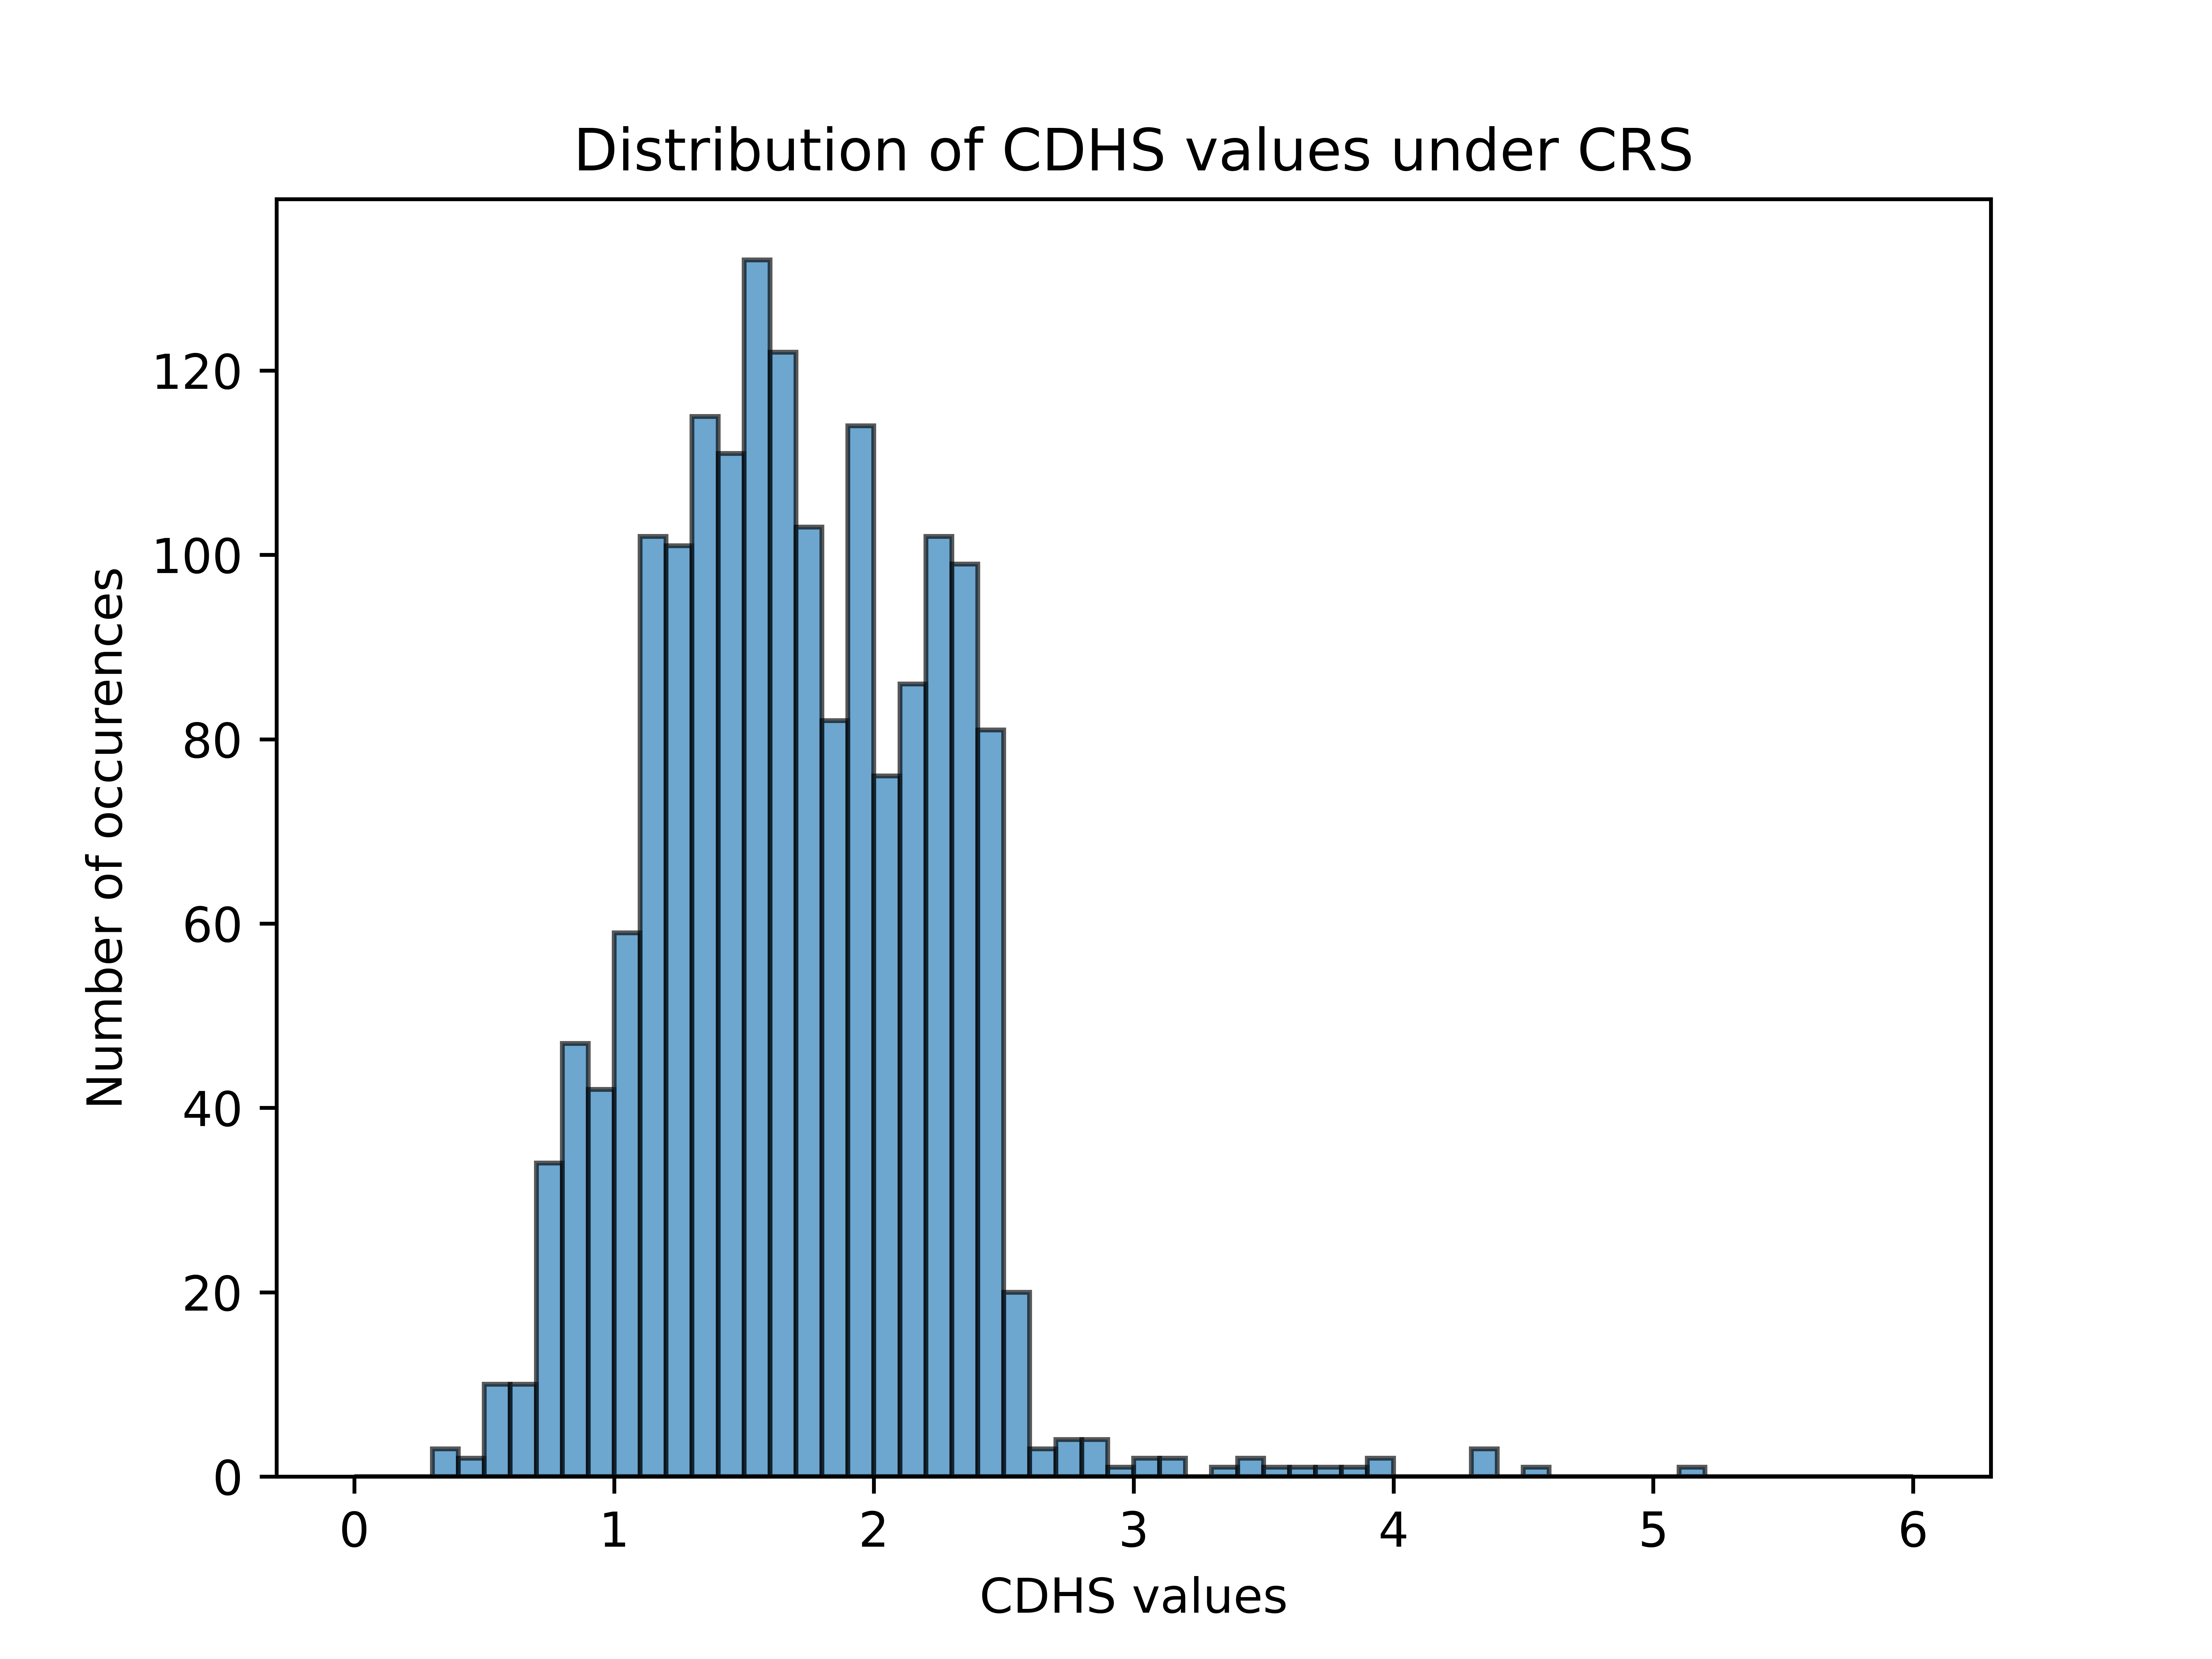
\includegraphics[width=\textwidth]{cdhs_crs.png}
    \caption{CDHS-CRS}\label{fig:distcdc}
  \end{subfigure}
  \qquad
  \begin{subfigure}[b]{0.3\textwidth}
    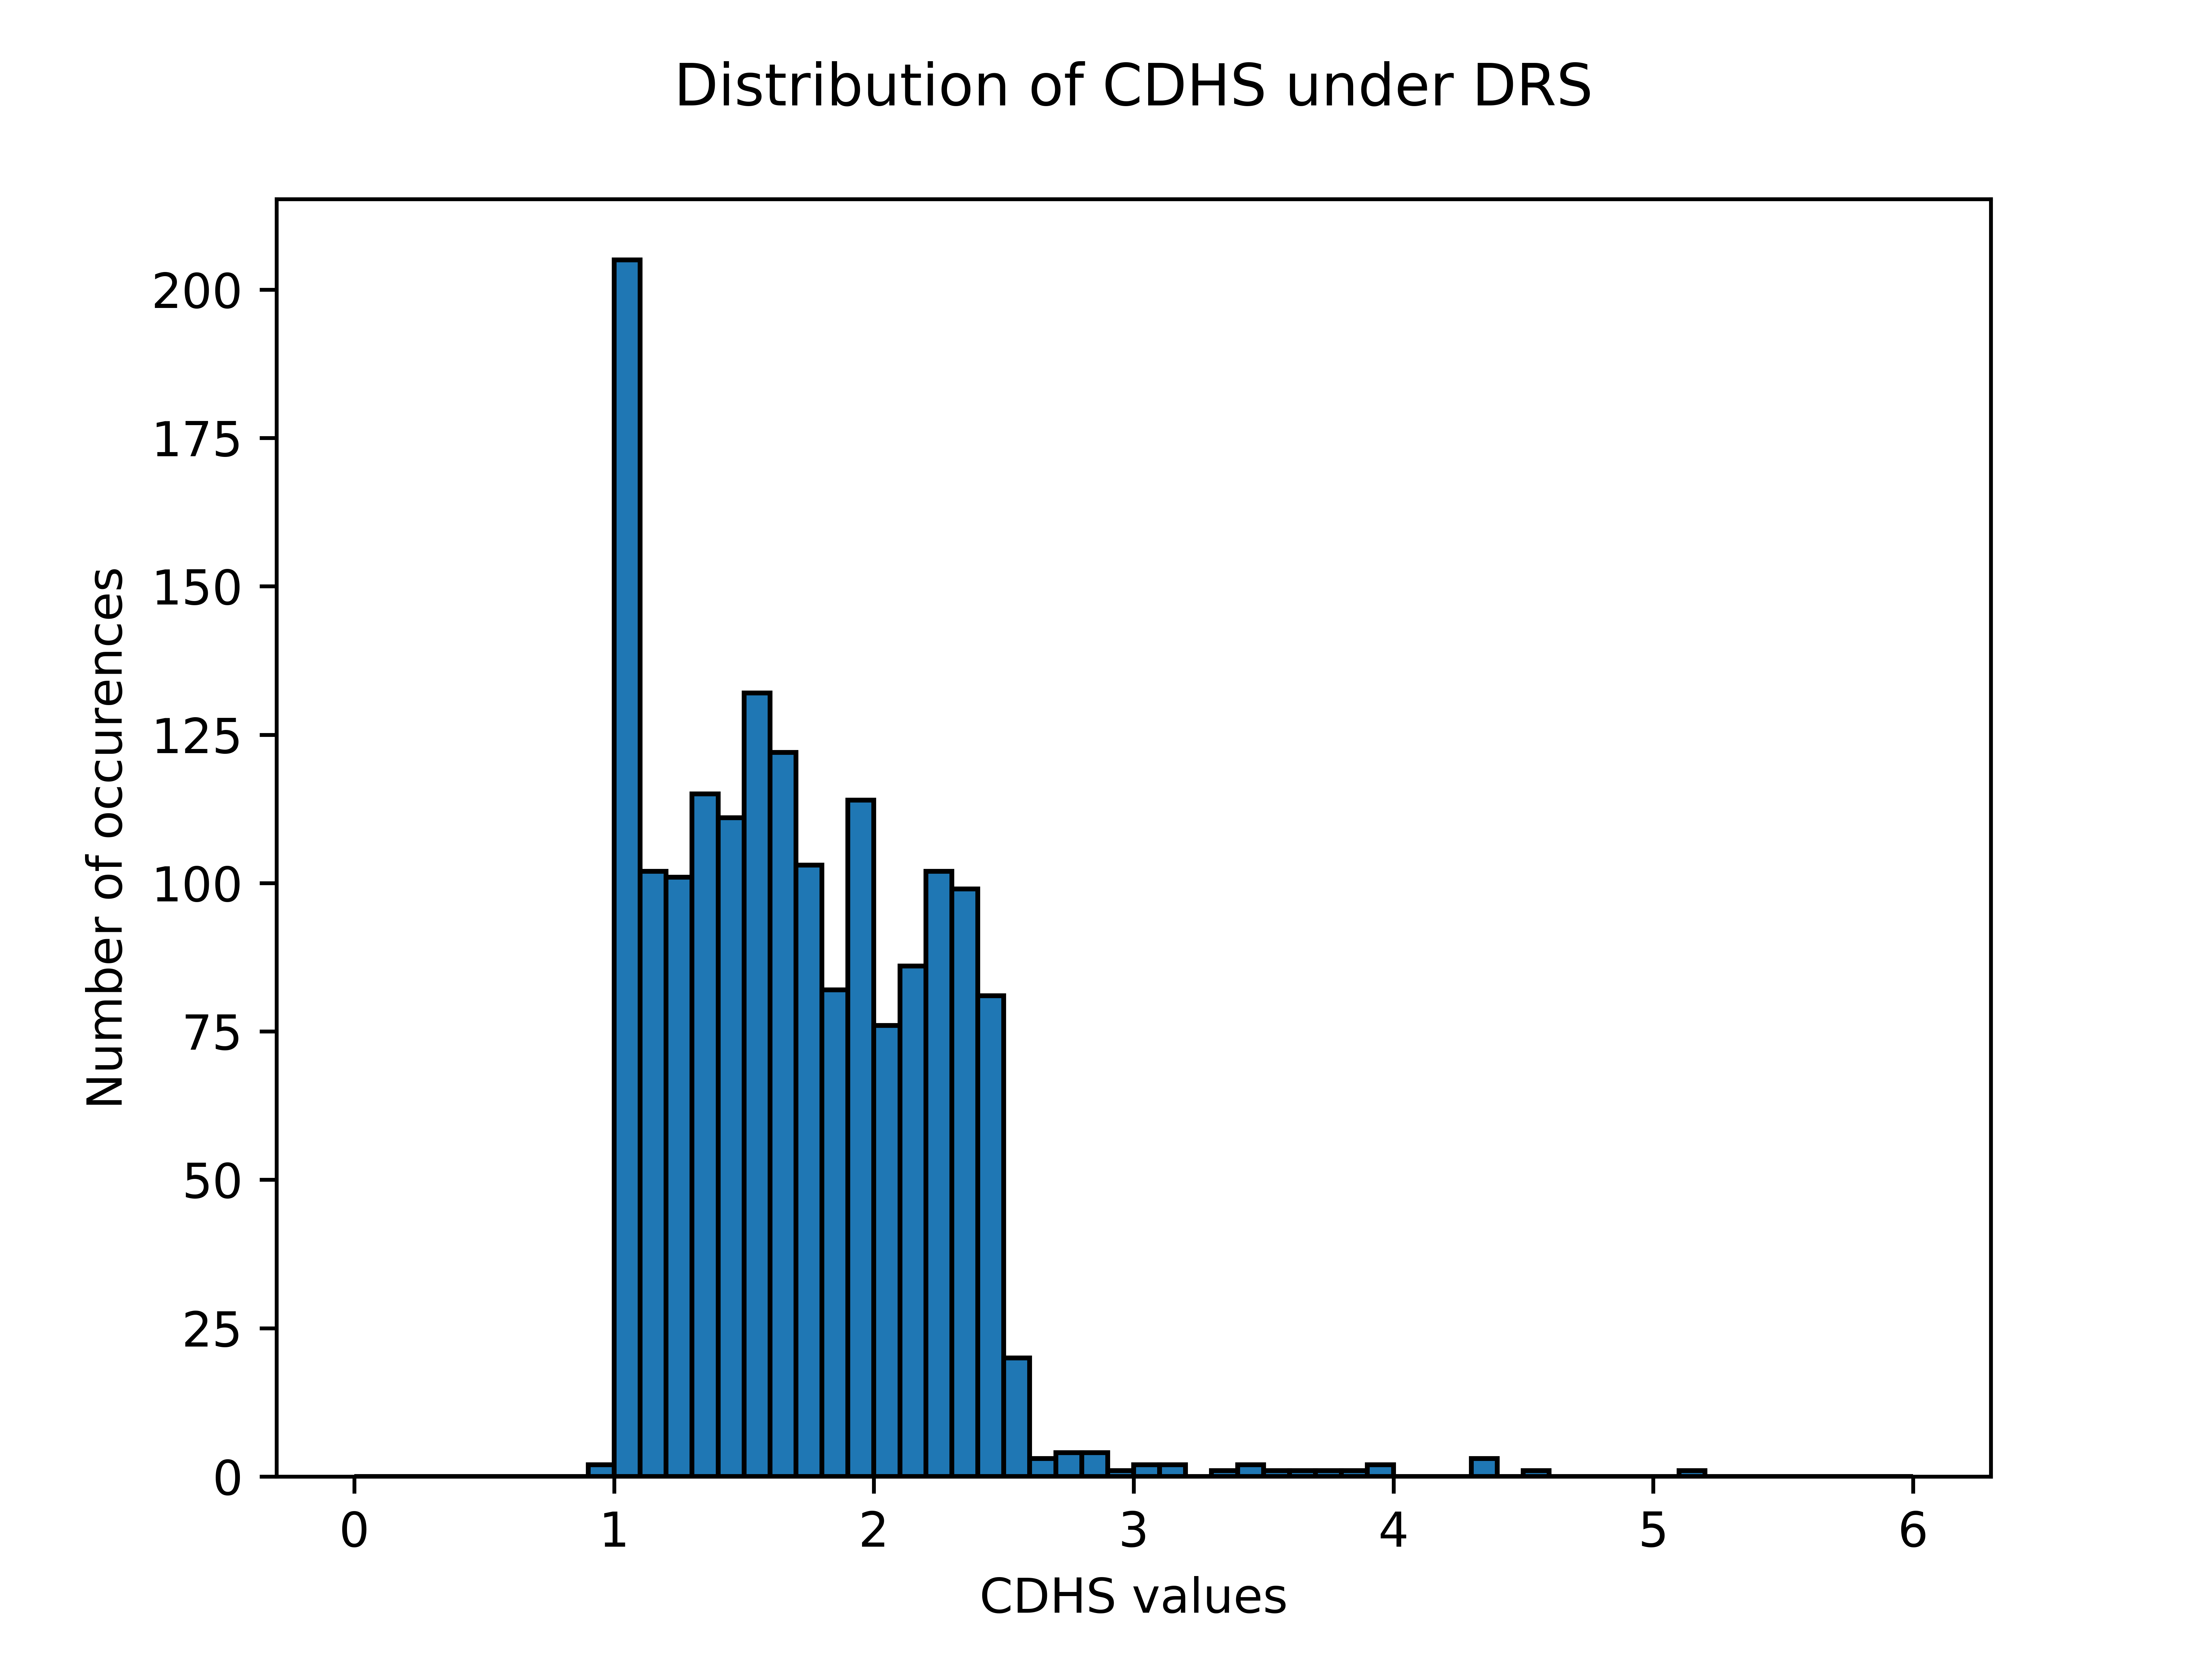
\includegraphics[width=\textwidth]{cdhs_drs.png}
    \caption{CDHS-DRS}\label{fig:distcdd}
  \end{subfigure}
  \caption{CDHS Distribution Plots}\label{fig:animals}
\end{figure}


\begin{figure}
  \centering
  \begin{subfigure}[b]{0.4\textwidth}
    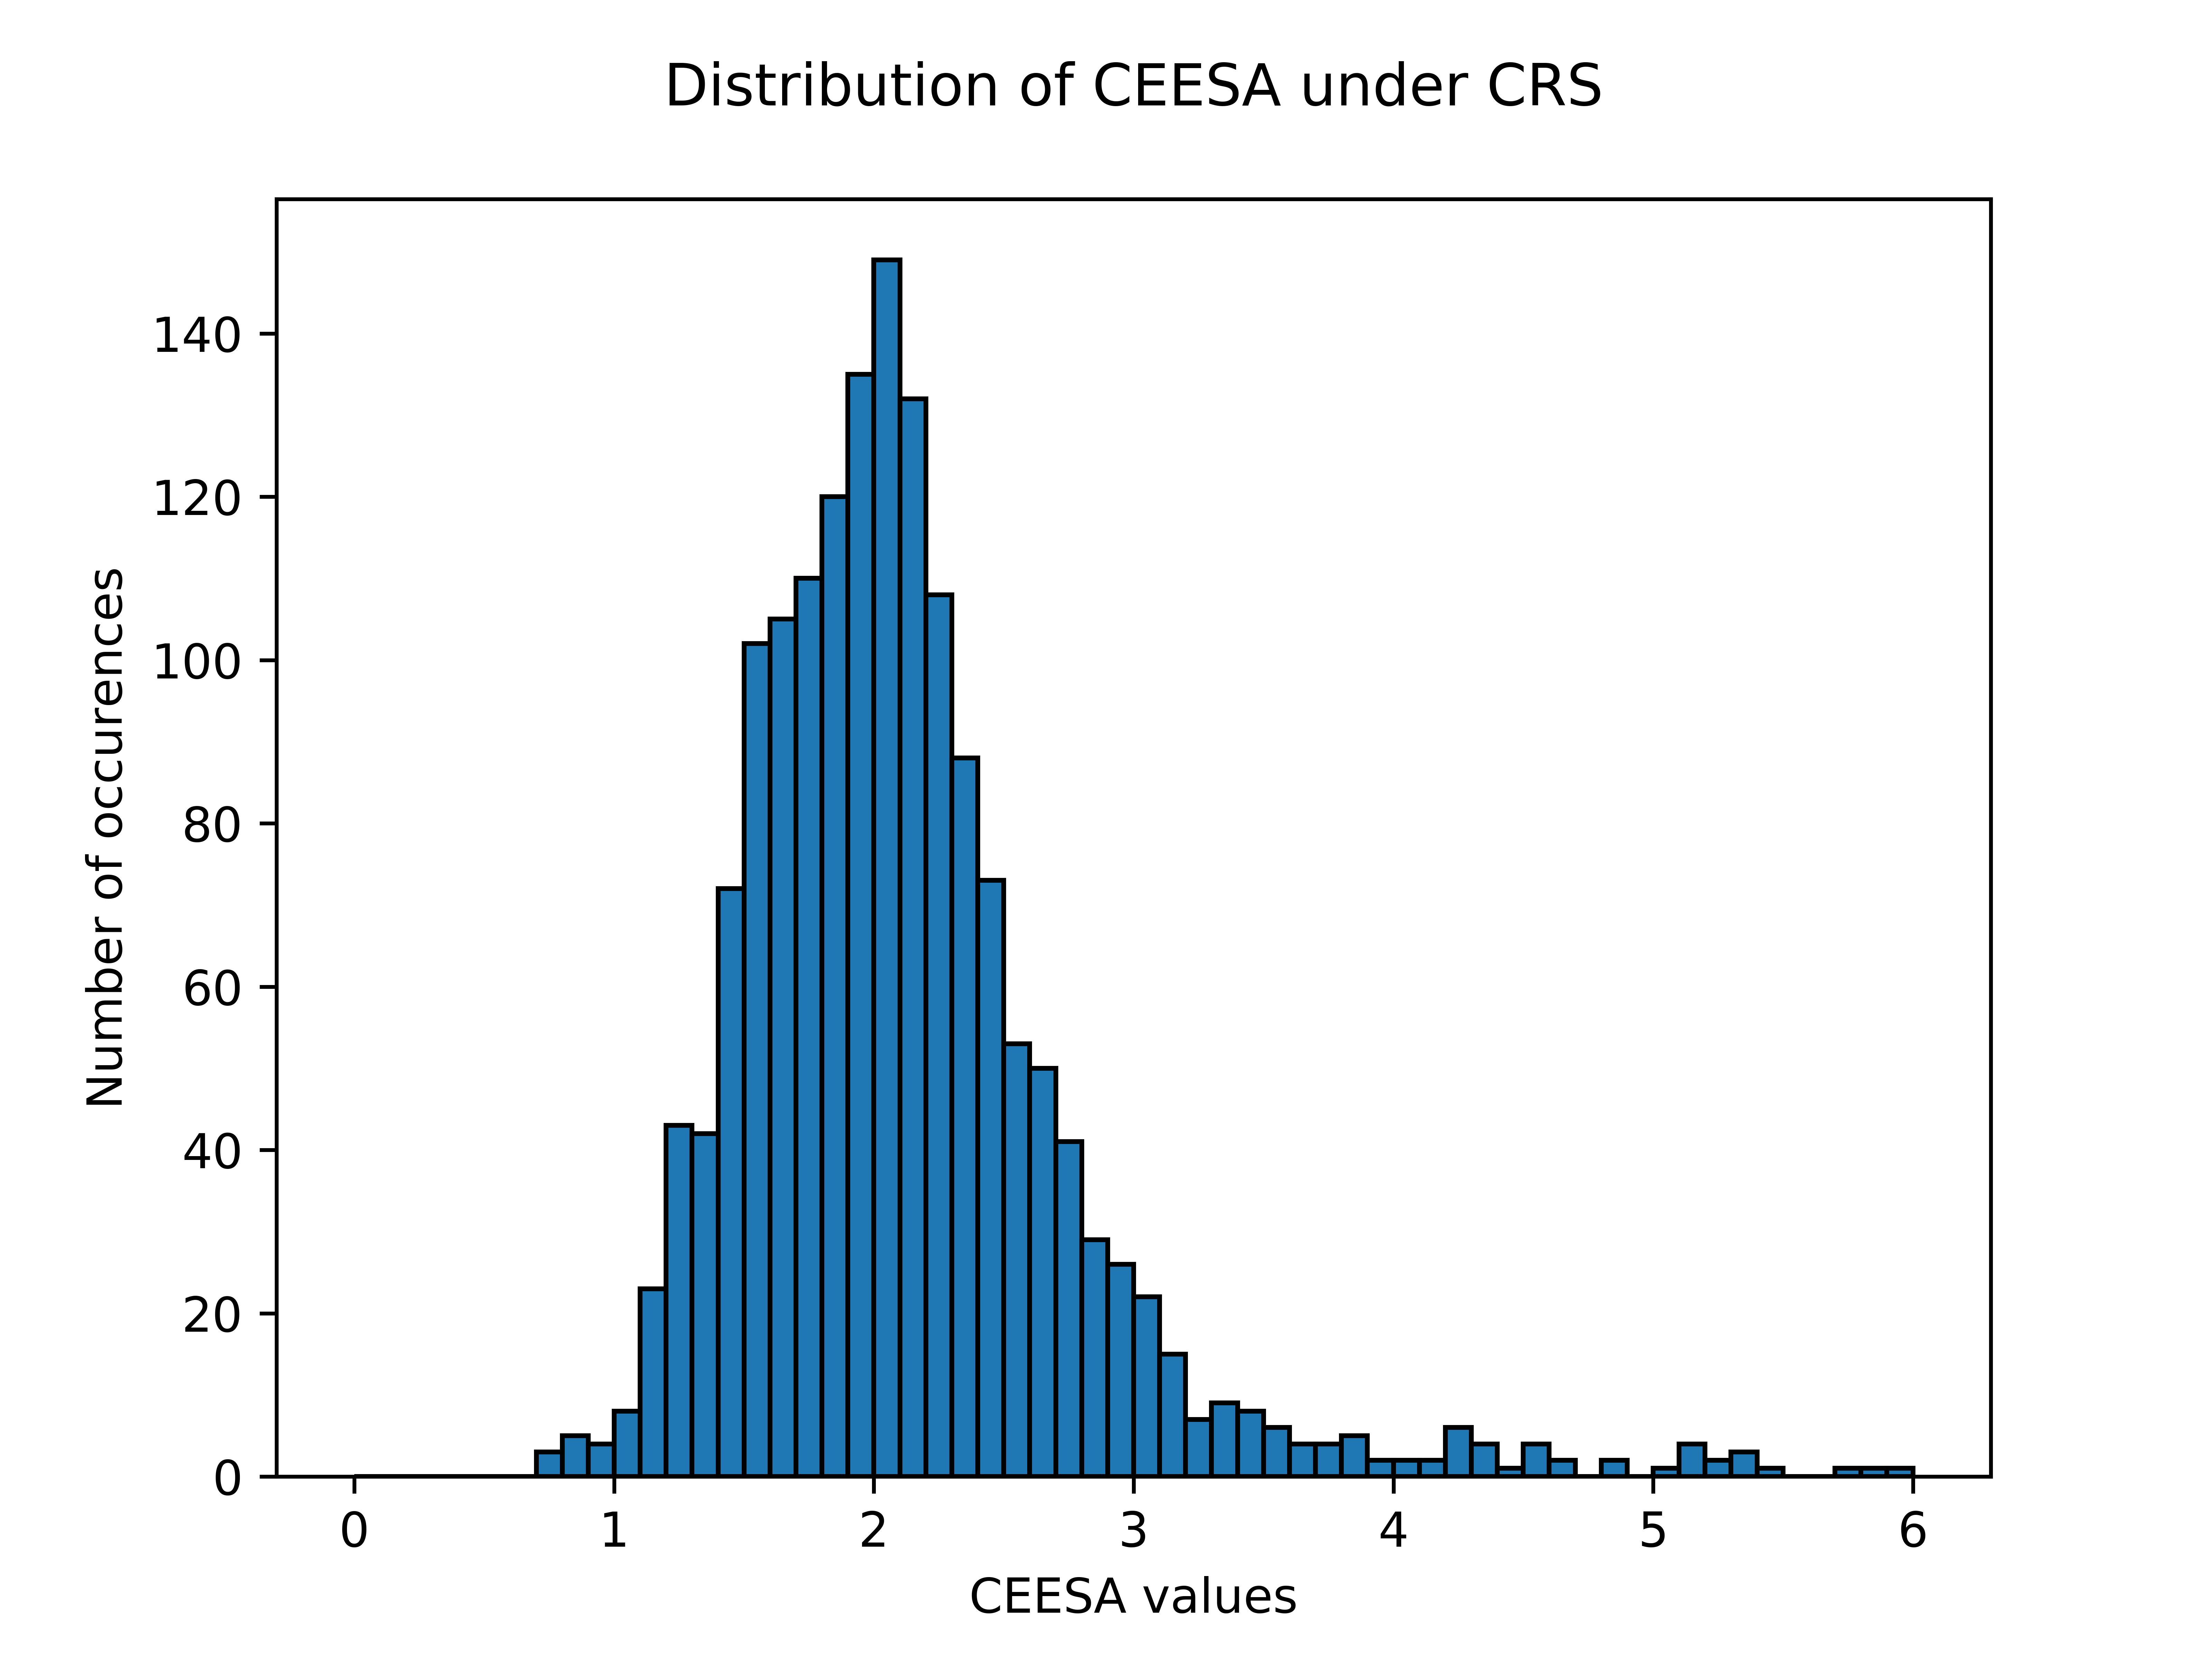
\includegraphics[width=\textwidth]{ceesa_crs.png}
    \caption{CEESA-CRS}\label{fig:distcdc}
  \end{subfigure}
  \qquad
  \begin{subfigure}[b]{0.4\textwidth}
    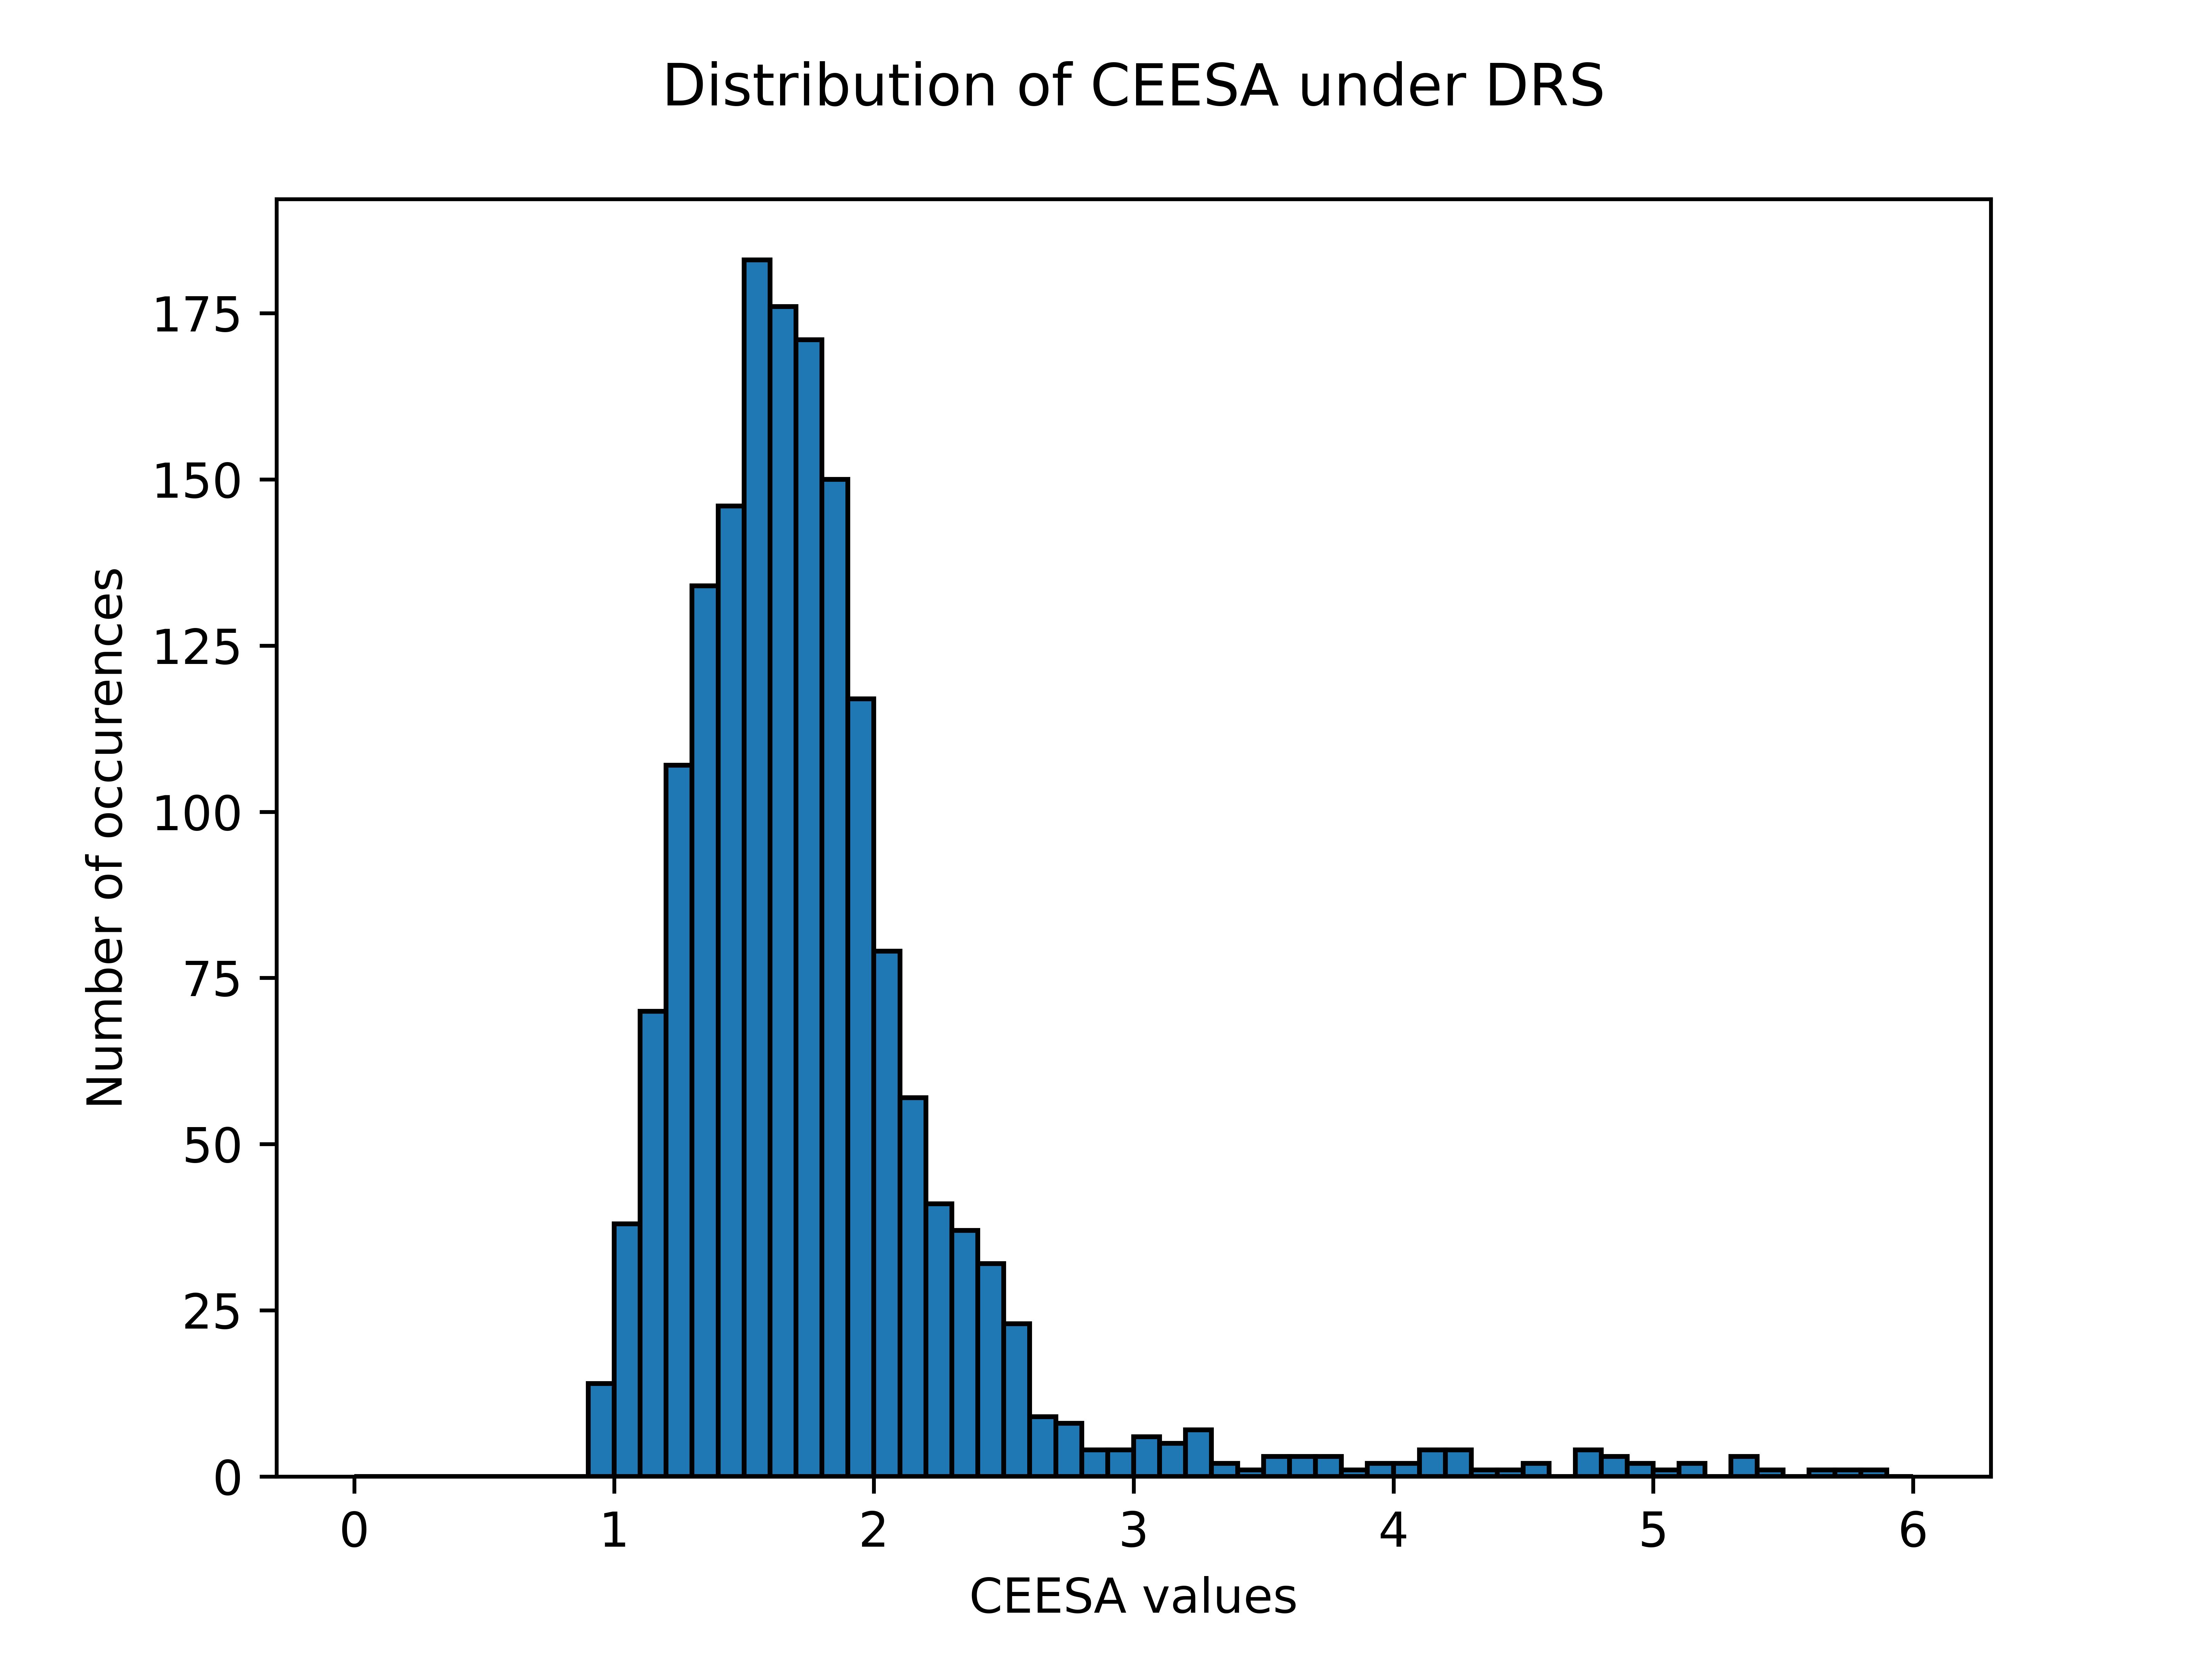
\includegraphics[width=\textwidth]{ceesa_drs.png}
    \caption{CEESA-DRS}\label{fig:distcdd}
  \end{subfigure}
  \caption{CEESA Distribution Plots}\label{fig:animals}
\end{figure}


\begin{figure}
  \centering
  \begin{subfigure}[b]{0.4\textwidth}
    \includegraphics[width=\textwidth]{iter_cdhs_crs.png}
    \caption{CDHS-CRS}\label{fig:distcdc}
  \end{subfigure}
  \qquad
  \begin{subfigure}[b]{0.4\textwidth}
    \includegraphics[width=\textwidth]{iter_cdhs_drs.png}
    \caption{CDHS-DRS}\label{fig:distcdd}
  \end{subfigure}
  \caption{CDHS Iterations Distribution Plots}\label{fig:animals}
\end{figure}


\begin{figure}
  \centering
  \begin{subfigure}[b]{0.4\textwidth}
    \includegraphics[width=\textwidth]{iter_ceesa_crs.png}
    \caption{CEESA-CRS}\label{fig:distcdc}
  \end{subfigure}
  \qquad
  \begin{subfigure}[b]{0.4\textwidth}
    \includegraphics[width=\textwidth]{iter_ceesa_drs.png}
    \caption{CEESA-DRS}\label{fig:distcdd}
  \end{subfigure}
  \caption{CEESA Iterations Distribution Plots}\label{fig:animals}
\end{figure}


% \begin{pointers}
% \item The values and proximity to earth's habitability score.
% \item Values that do not converge. Or were hard to converge.
% \item Speed of convergence graphs.
% \item Graph1: Iterations to convergence vs. Number of particles.
% \item Graph2: Distribution of number of iterations to convergence.
% \item Graph3: Iterations to convergence vs. Constraint parameters.
% \end{pointers}


\section{Conclusions}
\begin{pointers}
\item Why is the speed so important?
\item Parallelizable.
\end{pointers}


\appendix


\section{Improving Performance}\label{app:imp}

Matrices $P$ and $V$ represent current position and velocity, where the $i$\textsuperscript{th} row of each correspond
to the position and velocity of particle $i$. Each row of the matrix $L$ is the leader for the particle in the
corresponding row of $P$. The constraint matrix $C$ is constructed by stacking the constraint vectors $c_i$ described in
Section~\ref{sec:rep}. Let $r',r''$ be two random vectors of length $n$ drawn from the uniform distribution
${U(0,1)}^n$. Let $X_i$ denote the $i$\textsuperscript{th} row of matrix $X$. The implementation of each iteration while
updating particles in Algorithm~\ref{alg:cop} reduces to,

\begin{align*}
  g' &= f([\gbest])\\
  L  &= {[\argmin\limits_{pbest_j,\ j = 1\dots n} {\|pbest_j - P_i\|}^2\ \mid\ \forall i = 1\dots n\quad ]}^T\\
  V  &= \mu.V + \lambda_g\begin{bmatrix}
    {r_1}'(\gbest - P_1)\\
    {r_2}'(\gbest - P_2)\\
    \vdots\\
    {r_n}'(\gbest - P_n)
  \end{bmatrix} + \lambda_p\begin{bmatrix}
    {r_1}''(L_1 - P_1)\\
    {r_2}''(L_2 - P_2)\\
    \vdots\\
    {r_n}''(L_n - P_n)
  \end{bmatrix}\\
  V  &= [\quad\sgn(v_{ij})*\max\{|v_{max}|,|v_{ij}|\}\ \mid\ \forall i=1\dots n,\forall j=1\dots d\quad]\\
  P  &= P + V\\
\end{align*}

\end{document}
